\documentclass{book}

\usepackage[utf8]{inputenc}
\usepackage[T1]{fontenc}
\usepackage[catalan]{babel}
\usepackage{url}
\usepackage{hyperref}
\usepackage[numbers]{natbib}
\usepackage{wrapfig}
\usepackage{subfig}
\usepackage{sidecap}
\usepackage{verbatim}
\usepackage{setspace}

\usepackage[margin=2.5cm]{geometry}

\usepackage[pdftex]{graphicx}

\begin{document}

\pagestyle{empty}

\begin{titlepage}

\begin{center}


% Logo UAB

\includegraphics[width=1.00\textwidth]{./img/logoUAB.png}\\[1cm]    

% Title
\textsc{\LARGE Quadriga: Plataforma de Programació en Sistemes d'Entitats, per al desenvolupament de Videojocs.}\\[1.5cm]



\end{center}

\begin{flushright}

\vfill

% Dades
\begin{minipage}{0.4\textwidth}
\end{minipage}
\begin{minipage}{0.6\textwidth}
Memòria del Projecte Fi de Carrera \\
d'Enginyeria en Informàtica \\
realitzat per \\
{\bf Isaac Serrano Guasch} \\
i dirigit per \\
{\bf Enric Martí Godia} \\
Bellaterra, \today
\end{minipage}

\end{flushright}

\end{titlepage}
\newpage
% Logo UAB

\includegraphics[width=1.00\textwidth]{./img/logoUAB.png}\\[1cm]  

El sotasignat, Enric Martí Godia \\ \\
Professor de l'Escola Tècnica Superior d'Enginyeria de la UAB, \\ \\
{\bf CERTIFICA:} \\ \\
Que el treball a què correspon aquesta memòria ha estat realitzat sota la
seva direcció per en Isaac Serrano Guasch. \\ \\
I per tal que consti firma la present. \\ \\
\newpage
\newpage

{\LARGE Agraïments}
\\

Primer, a en Jordi Arnal per a guiar-me a sistemes semblants al que volia desenvolupar, però ja acabats, i no tallar-se un pèl a l'hora de senyalar defectes al meu.
\\

Als meus companys del Màster de Creació de Videojocs: en Sergi, n'Hèctor, en Carles, n'Eduard, n'Albert i en José Manuel, per ajudar-me a viure un projecte més real i fer-me veure quines són les seves necessitats, i als professors del mateix Màster per donar-me les eines per resoldre-les.
\\

I finalment, a la meva parella, n'Ada, per repassar aquesta memòria quan calia, la meva família i als meus amics per acompanyar-me i animar-me en el trajecte de la carrera del qual aquest projecte n'és només l'estació final.

\pagestyle{headings}
\setcounter{page}{1}
\pagenumbering{roman}

\tableofcontents
\listoffigures
\listoftables


\chapter{Introducció}

Des de l'aparició dels primers videojocs, la seva evolució ha estat sempre emparellada amb una evolució tecnològica constant i, en certs punts, accelerada. Aquesta evolució tecnològica no només consta de millores en el rendiment i qualitat de cada joc sinó que, a més, s’han aconseguit generalitzar solucions i aplicar la tecnologia d’un videojoc a d'altres i fins i tot crear eines que permeten el desenvolupament de jocs a partir d'elles.

Si mirem aquesta evolució des de més a prop, veiem com al principi els videojocs eren evolucions d'altres jocs típics de bar. Màquines escurabutxaques com el pinball serviren d'inspiració per a crear els primers videojocs comercials, amb un model de negoci molt semblant. Posteriorment, la necessitat de crear grans quantitats de jocs va obligar als desenvolupadors a crear màquines que poguessin executar més d'un joc i així abaratir costos. Tot això passava sobretot a la dècada dels setanta i principis dels vuitanta. Però finalment, amb l'arribada dels ordinadors personals i les consoles de sobretaula, es comença a desenvolupar un mercat per a jocs sobre plataformes genèriques.

A poc a poc van apareixent els motors gràfics - programes o mòduls encarregats del renderitzat d'un joc o d'un programa amb gràfics 2D o 3D - o fins i tot motors de joc - una plataforma per desenvolupar-hi un joc a sobre -. En un principi aquests motors s'utilitzaven dintre de la mateixa companyia que el creava. Per exemple LucasArts creà {SCUMM} ({Script Creation Utility for Manic Mansion}) \citep{WikiScumm} a l'hora que creava la seva aventura gràfica de "Point \& Click" Manic Mansion (1987). Aquest mateix programa fou utilitzat després en d'altres jocs com Indiana Jones i l'Última Creuada, LOOM, El Dia del Tentacle i tres jocs de la saga Monkey Island (fins al 1998).

Un pas més endavant el va dur Id Software amb el seu {\em id Tech}  \citep{WikiScumm}. Aquest motor - i les seves evolucions - no només es feu servir per fer jocs com Doom (1993) i Doom II (1994) d'Id Software, sinó que es va vendre a altres companyies per a fer altres jocs, tot i que aquests jocs serien molt semblants al Doom original, com serà el Half-Life (1998) basat en el Quake engine, una evolució de l'{\em id Tech}. Posteriorment fins i tot hi va haver companyies que basaven el seu negoci no en vendre jocs, sinó en vendre motors a altres companyies que els fessin servir; és doncs l'aparició definitiva dels motors com a Middleware.

Paral·lelament a l'evolució tecnològica ja esmentada, la metodologia de desenvolupament i els mateixos llenguatges de programació han anat evolucionant. L'evolució més important fou quan es va passar de programar bàsicament en {\bf C} a {\bf C++}. El canvi de paradigma, però, s'ha demostrat difícil i, tot i que l'ús de la metodologia orientada a objectes és predominant a quasi totes les àrees d'un motor, encara n'hi ha alguna on s'ha demostrat no ser la millor solució. A la figura \ref{fig:EsquemaEngine} es mostren algunes parts d'un {\em Engine} i com el mòdul de lògica usa els altres. D'aquesta manera un pot imaginar-se un {\em Engine} com a un proveïdor de serveis per al mòdul de lògica.


\begin{figure}
  \centering
  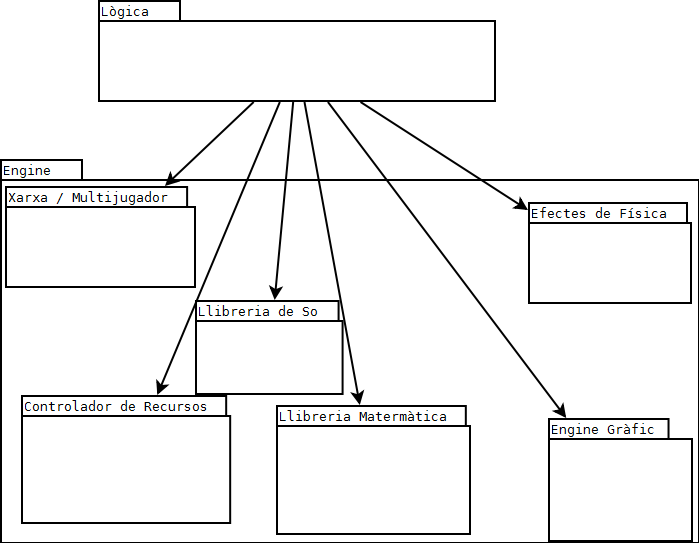
\includegraphics[width=0.58\linewidth]{./img/EsquemaEngine.png}
  \caption{Esquema genèric d'un Engine \label{fig:EsquemaEngine}}
\end{figure}

L'àmbit on més canvis hi ha hagut, en quan a metodologia de desenvolupament, i el que en aquest treball ens centrarem és en la definició de la lògica d'un joc. Les lògiques dels jocs, també conegudes com a mecàniques, són les normes que defineixen els jocs. Aquestes normes estan compostes per diverses peces: elements interactius i no interactius (com l'escenari del joc, els personatges, {\em attrezzo}, i altres), accions que poden fer els elements interactius i els objectius que té el jugador.

En aquest capítol s'explicarà primer l'evolució històrica en quan a programació de la lògica dels jocs. Seguidament agafarem la mostra que volem implementar i la definirem, i es mostraran alguns exemples de jocs i {\em Engines} que han implementat solucions semblants. Finalment s'esmentaràn els objectius d'aquest projecte.

\section{Evolució en les mecàniques dels jocs}

 En aquesta secció s'explicarà l'evolució que han anat prenent els mètodes que tenen els desenvolupadors per a definir aquestes normes; des de l'aproximació clàssica, jeràrquica i intuïtiva, agrupant els elements per característiques comunes, seguida d'un replantejament estructural, on se segueix una arquitectura menys intuïtiva, però més flexible, sense definir jerarquies de elements, amb característiques comunes, sinó definint cada característica per separat i després deixant que cada element agrupi les que necessita. I finalment presentant una arquitectura que trenca per complet l'aproximació clàssica sense deixar de ser una evolució del pas anterior.

\subsection{L'aproximació clàssica}

Quan un programador de {C++} o de qualsevol llenguatge orientat a objectes s'asseu davant el desafiament de programar la lògica d'un joc, llista les diferents entitats del joc (escenari, jugador, enemics, armes, etc.) i els distribueix en diferents grups i subgrups. Després en programa les funcionalitats comunes i acaba creant una jerarquia de classes que defineixen totes les entitats i les seves interrelacions. 

Aquesta aproximació sembla senzilla, però acaba comportant diversos problemes. Com s'explica a \citep[p.~719]{Gregory09}, les jerarquies de classes massa grans pateixen dels següents inconvenients:




\begin{itemize}
  \item {\bf Manteniment:} A més profunda és una classe dintre d'una jerarquia, més costa d'entendre, mantenir i modificar, ja que s'ha d'entendre tant ella com totes les seves classes superiors. Per exemple el fet de modificar una funció virtual aparentment innòcua, pot comportar trencar suposicions que faci alguna de les classes mare, cosa que du a errors subtils i difícils de detectar.
    
  \item {\bf Impossibilitat de descriure taxonomies multi-dimensionals:} Crear classes en forma d'arbre és molt pràctic i sobretot intuïtiu, especialment on a cada nivell es fan separacions respecte un criteri per cada nivell. Inicialment, ens plantegem una llista de grups a classificar: Vehicles contra Animals, Terrestres contra Marítims, etc. Aquí se'ns obra el primer dilema: Classifiquem primer entre animals i vehicles, o entre terrestres o marítims? Però el problema seriós arriba quan ens trobem amb classificacions que no havíem previst inicialment. Per exemple podríem havent classificat vehicles terrestres i aquàtics (figura \ref{fig:Vehicles}), i posteriorment podem haver d'afegir vehicles amfibis, repte que es pot intentar solucionar de les següents maneres:
  
  \begin{figure}
    \centering
    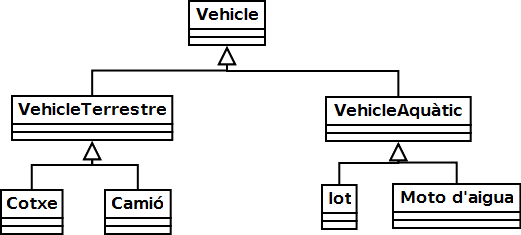
\includegraphics[width=0.58\linewidth]{./img/Vehicles.png}
    \caption{Vehicles classificats en terrestres i aquàtics \label{fig:Vehicles}}
  \end{figure}
  
    \begin{enumerate}
      \item {\bf Crear una nova classe hereva de vehicle \"{}VehicleAmfibi\"{}:} Solució òptima a primer cop d'ull, però comporta duplicar codi, ja que el codi necessari per fer que un vehicle vagi per terra ja es troba a {\em VehicleTerrestre}, per exemple. Això ens du a intentar la segona solució.
      
      \item {\bf Herència múltiple. El diamant de la mort:} La solució naïf del problema anterior seria crear la classe {\em VehicleAmfibi} hereva tant de {\em VehicleTerrestre} com de {\em VehicleAquàtic}, cosa que ens porta directament a l'herència múltiple. Com s'explica a \cite[p.~2]{Martin97}, l'herència múltiple causa diversos problemes, moltes vegades més grans que aquells que soluciona. Per exemple en aquest cas veuríem que la classe {\em VehicleAmfibi} heretaria dues vegades {\em Vehicle}, amb els problemes d'ambigüitat que això duria (figura \ref{fig:RombeMort}).
        
        
      \begin{figure}
        \centering
        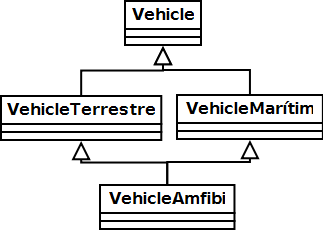
\includegraphics[width=0.58\linewidth]{./img/RombeMort.png}
        \caption{Diamant de la mort \label{fig:RombeMort}}
      \end{figure}
        
      \item {\bf Classes Mix-in:} Una altra solució per crear taxonomies multi-dimensionals és crear un seguit de classes que aportin funcionalitat a diversos llocs de la jerarquia. Aquestes classes, per funcionar bé, cal que siguin heretades només per les fulles i que cap d'elles tingui una classe mare. Per tant diríem que una classe només pot tenir un "avi" en qualsevol cas. Aquesta solució comporta, sobretot, molta disciplina i acaba resultant en una solució molt semblant a "agregar" funcionalitat en comptes d'heretar-la (figura \ref{fig:MixIn}).
        
      \begin{figure}
        \centering
        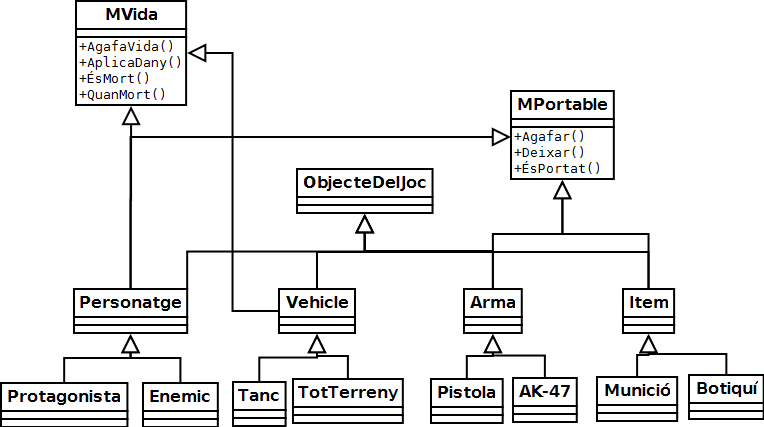
\includegraphics[width=0.58\linewidth]{./img/MixIn.png}
        \caption{Esquema amb classes \"{}Mix-In\"{} \label{fig:MixIn}}
      \end{figure}
    \end{enumerate}
    
  \item {\bf Efecte bombolla:} A l'inici del disseny, les classes arrels - les més pròximes a l'inici de la jerarquia - són dissenyades inicialment amb poca funcionalitat. A mesura que avança el projecte, i davant del desig de compartir codi (i sobretot, no duplicar-lo), molta funcionalitat va pujant a la jerarquia fins que troba el \"{}comú denominador\"{}. A poc a poc, les classes arrels es van fent pesades fins que contenen la major part de funcionalitat, que les seves filles s'han d'encarregar d'activar correctament. Col·lateralment això fa que moltes classes acabin tenint una funcionalitat i unes variables que realment no necessiten, fent que el programa usi més memòria de la necessària, un problema especialment greu en jocs de consola, on la memòria és un bé molt escàs.
    
    
  
\end{itemize}

Per a més informació sobre els defectes de l'aproximació clàssica, consultar \cite{Wilson02}.

\subsection{De l'{\em és-un} al {\em conté-un}}

La primera millora, o petit canvi, que es proposa respecte l'aproximació anterior, és agregar la funcionalitat en comptes d'heretar-la. Si es vol crear un objecte amb moviment, que es renderitzi, que col·lisioni i que s'animi - un enemic, per exemple -, en l'aproximació clàssic la classe que representa aquest objecte heretaria d'una jerarquia on, més amunt o més avall, estigui implementada tota aquesta funcionalitat (figura \ref{fig:EnemicHerencia}). La millora proposada consta de fer que aquesta classe contingui aquelles que ens aportin cada una la funcionalitat que busquem (figura \ref{fig:EnemicAgregacio}).

\begin{figure}
  \centering
  \subfloat[Estructura per herència]{\label{fig:EnemicHerencia}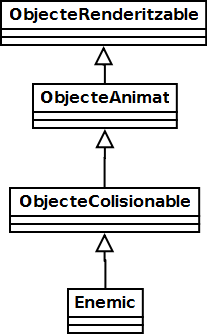
\includegraphics[width=0.23\textwidth]{./img/EnemicHerencia.png}}
  \hspace{0.08\textwidth}
  \subfloat[Estructura per composició]{\label{fig:EnemicAgregacio}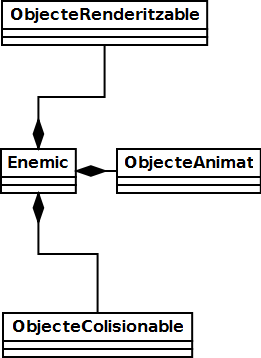
\includegraphics[width=0.27\textwidth]{./img/EnemicAgregacio.png}}
  \caption{Comparació d'herència i composició. \label{fig:HerenciaAgregacio}}
\end{figure}

Dintre d'aquest esquema, les classes que aporten funcionalitat són moltes vegades anomenades {\em Components} o {\em objectes-servidors}, ja que són les que componen els objectes finals.

Aquesta aproximació millora en certs aspectes l'anterior, com es mostra més endavant a la taula \ref{tab:comparacioFilosofies}, però encara té alguns inconvenients. Es tendeix a tenir una classe {\em GameObject} amb un punter a cada tipus de component, al qual se li afegeixen o treuen els components segons convingui - un {\em Enemic} contindrà el component {\em ObjecteAnimat} mentre que una {\em Habitació} no -; cosa que comporta primer el problema de qui s'ha d'encarregar de destruir els components - evident fins que arribes al punt que vols substituir un component en temps d'execució - i després la pèrdua d'eficiència que comporta haver de comprovar constantment si una instància conté o no cada component per fer-ne operacions.

Un pas més enllà es troba l'aproximació on cada tipus de {\em Component} implementa una interfície comuna molt bàsica i després el {\em GameObject} simplement conté un array dinàmic que els conté tots, i crida les seves funcions ordenadament. Aquesta aproximació comporta sovint el problema de que els components cal ordenar-los, ja que moltes vegades la seva funcionalitat no és commutativa.

Un últim pas en aquesta línia és eliminar per complet el {\em GameObject} i tenir arrays de components i lligar-los simplement per l'índex; Arrays o una implementació menys costosa en memòria com Taules Hash. Aquesta aproximació sovint anomenada com a {\em Model de Components Pur} \citep{Martin07} guanya sobretot en localitat de memòria. Normalment tots els components d'un tipus s'actualitzen alhora, en estar tots seguits en un array, el programa troba totes les dades juntes i s'executa més ràpidament que si les dades estiguessin dispersades.

Finalment, un gran avantatge d'un sistema d'aquest tipus és, com s'explica a \citep{Leonard99}, la possibilitat de, un cop definits els tipus de components i les seves propietats, crear un \"{}editor del joc\"{} que permeti, amb l'ajuda d'una interfície gràfica, crear, manipular, modificar, afegir, treure, etc. objectes i components del món de forma molt senzilla. Una eina d'aquestes característiques disminueix la dependència que hi ha entre dissenyadors i programadors i permet que cada un d'ells pugui fer la seva feina en paral·lel de la forma més eficient possible.

\subsection{De centrar-nos en els objectes, a centrar-nos en les propietats}

L'últim pas, que abstreu totes les idees anteriorment exposades, és trencar totalment l'esquema orientat a objectes. Aquest canvi s'inspira en part en l'arquitectura Model-Vista-Controlador. Concretament n'agafa el concepte de que cal separar les dades de la lògica que les controla. Si en féssim una base de dades hauríem de primer llistar tots els tipus de propietats que una entitat del joc pot tenir; de cada element d'aquesta llista l'anomenarem {\bf Component}, ja que les esmentades entitats seran formades a partir d'aquests. D'aquesta manera podem crear una taula per cada tipus de component que una entitat del joc pot tenir, i fer-ne una columna per cada propietat i una fila per cada objecte que el contingui, tenint cada objecte del joc, el que abans coneixíem com un {\em GameObject}, un identificador únic.

Aquesta aproximació no està pas mancada de defectes, i cal tenir-los en compte. El primer d'ells és la dificultat que hi ha d'establir relacions entre les {\em entitats} del joc, ja que no existeix una implementació en sí, d'aquesta entitat. Relacionat amb això hi ha el problema d'inicialitzar aquestes {\em entitats}, que s'ha de fer d'una forma més o menys aliena al mateix sistema. Finalment, el dilema més gran, és decidir on es programa el comportament de les entitats. Hi ha bàsicament 2 solucions, amb les seves variants:

\begin{enumerate}
  \item {\bf Dintre els mateixos components:} Cada propietat porta incorporada la seva funcionalitat d'alguna manera. Sigui directament dintre del mateix component, via mètodes en aquest - cosa que retorna a la metodologia orientada a objectes - o via els anomenats {\em sistemes}. Aquests s'encarreguen de recollir aquelles {\em entitats} que reuneixen unes condicions - normalment, tenir un o més components - i actualitzar-los.
    
  \item {\bf Via components especials:} En aquesta variant normalment es defineix un tipus especials que simplement conté un apuntador - o referència equivalent - a un script que implementi una interfície coneguda i que defineixi el comportament d'aquesta entitat.
    
\end{enumerate}

Finalment podem veure a la taula \ref{tab:comparacioFilosofies} una comparació de les característiques de cada arquitectura.

\begin{table}
  \begin{tabular}{ | p{0.15\textwidth} | p{0.20\textwidth} | p{0.20\textwidth} | p{0.40\textwidth} | }
    \hline
     &
     {\bf Manteniment} &
     {\bf Impossibilitat de descriure taxonomies multi-dimensionals} &
     {\bf Dependències externes} \\
     \hline
     
     {\bf Aproximació clàssica} &
     A més complexitat del sistema, més difícil és de modificar o ampliar. &
     Un cop s'han decidit quins atributs seran diferenciadors en cada punt de la jerarquia, canviar-los porta problemes. &
     Si volem modificar una dependència (per exemple, canviar la llibreria de física) caldrà modificar aquelles classes que encapsulin la física i adaptar totes aquelles hereves i en conseqüència cal fer molts canvis al programa, especialment si hi ha entitats que no fan servir aquesta característica però la duen incorporada, degut a l'efecte bombolla.\\
     \hline
     
     {\bf Composició de Propietats} &
     La complexitat vé relacionada amb la quantitat d'interrelacions entre les propietats, no amb el nombre total de propietats. &
     Una entitat pot ser reclassificada en qualsevol moment, i l'ampliació de classificacions no afecta a les ja existents. &
     A l'hora de modificar una llibreria externa només cal tocar els components que la necessitin i, si hi ha un canvi prou gran, les entitats que els continguin. \\
     \hline
     
     {\bf Separar les dades de la Lògica} &
     El sistema té una arquitectura més complexa, però al minimitzar les dependències és la més flexible. &
     Exactament igual que en el cas anterior. &
     Al dissenyar les dades del joc de forma independent de la seva implementació, aquesta es pot canviar sense més conseqüències. \\
     \hline
  \end{tabular}
  \caption{Comparació entre diferents arquitectures. \label{tab:comparacioFilosofies}}
\end{table}

\section{Sistema d'Entitats}

En aquesta secció donarem una definició, la nostra, del que és un sistema d'entitats. Tot seguit, es mostraran diferents implementacions que s'han fet, tant de Videojocs com d'{\em Engines}.

\subsection{Definicions}

Un sistema d'entitats està compost de diferents elements que cal entendre.

En primer lloc, les {\bf entitats}. Una {\bf entitat} en un videojoc és cada element que d'alguna manera apareix en el videojoc de forma concreta. Per exemple, l'escenari del videojoc, l'{\em avatar} del jugador, els enemics, les armes, els objectes que el jugador recull. Si féssim un llistat exhaustiu del joc dels escacs, donaríem les peces, el taulell i, si s'escau, el rellotge que marca el temps límit.

Seguidament, els {\bf components} són les característiques que defineixen les {\em entitats}. La vida d'un personatge, el model 3D de l'escenari i la velocitat d'un cotxe en són exemples, però també n'hi ha de més abstractes, com un component que defineix que un objecte fa so, o un altre que el marca com a {\em vehicle}. En resum, totes les característiques que les {\bf entitats} poden tenir s'agrupen en {\bf components}.

Finalment definim un {\bf sistema d'entitats} aquell {\bf sistema} que regeix el comportament d'un seguit d'{\bf entitats}, definides a partir d'uns {\bf components}. Cada entitat té associat com a màxim un component de cada tipus. El comportament d'aquestes entitats ve únicament regit per quins {\bf components} té associats i les dades que aquests contenen.

\subsection{Implementacions}

En aquesta secció farem un repàs de diverses implementacions de sistemes d'entitats que s'han fet anteriorment, analitzarem les seves característiques i els avantatges i inconvenients d'alguns.

Començarem amb un anàlisi d'alguns jocs que han seguit aquesta aproximació, seguidament parlarem de motors de jocs i finalment parlarem del nostre motor, i quines característiques tindrà que el diferenciïn dels anteriors.

\subsection{Jocs}

És difícil de rastrejar quins jocs tenen una estructura d'agregació en comptes d'herència, ja que moltes vegades no es fa pública la implementació d'aquestos. Però gràcies als anomenats {\em postmortemps} (Documents que s'escriuen un cop finalitzat un joc, on se n'analitza el desenvolupament, es busquen quines coses han anat bé i quines no i s'intenta fer auto-crítica de cara a millorar el desenvolupament dels següents projectes) podem tenir accés a la informació d'alguns jocs. A continuació una breu mostra d'alguns d'aquests, amb la referència d'on se'n poden trobar més detalls.

\begin{description}
  \item[Thief] \citep{Leonard99} Potser un dels exemples més antics, encara que segurament no el més antic, ja que el sistema és sempre una evolució d'algun motor usat anteriorment. Basa la seva força en facilitat d'edició mitjançant GUIs i una alta versatilitat, desenvolupant 2 jocs en paral·lel bona part del temps ({\em Thief} i {\em System Shock 2}). Es destaca que en aquests jocs no hi ha cap jerarquia d'objectes en el codi, sinó que tota es crea a partir de dades.
    
  \item[Tony Hawk's Pro Skater 3] \citep{West07} En aquest exemple veiem la necessitat d'una companyia de treure jocs amb una alta freqüència (un a l'any) i com, a poc a poc evolucionant cap a un sistema d'entitats fetes amb agregació de components. El canvi de jerarquies en el codi a objectes creats via dades fou lent i al principi contraproduent, però 2 anys després de començar el canvi els resultats es feren evidents, on el joc va guanyar en velocitat d'execució i els creadors en temps de producció.
    
  \item[Dungeon Siege] \citep{Bilas02} Potser dels més coneguts, sinó el més referenciat, Dungeon Siege anava equipat amb un sistema de components que permetia crear aquests components tant en {\em C++} com amb {\em Skirt}, un llenguatge propi del joc. Aquesta flexibilitat, i una aproximació a les dades molt similar a una Base de Dades Relacional va cridar molt la atenció a la GDC de San José (Un congrés de creadors de videojocs), potser quan els sistemes d'entitats van començar a agafar nom a la indústria.
    
\end{description}


\subsection{Motors de jocs}

Diversos motors de jocs han seguit aquesta filosofia, tant comercials, oberts o híbrids. En repassarem alguns.

\begin{description}
  \item[Unity] (\url{http://unity3d.com/}) Probablement el motor més ambiciós disponible sota aquesta filosofia. Seguint un model de negoci híbrid, ja que pots fer servir una versió limitada de forma gratuïta i accedir a diverses millores pagant, Unity aporta sobretot un editor molt potent, que permet fer gairebé qualsevol cosa que necessites des del mateix editor i veure com queda al joc quasi en temps real. Aquesta aproximació redueix moltíssim els temps de producció i facilita la feina sobretot als dissenyadors, per la facilitat que dóna a prototipar dissenys.
    
  \item[Frostbite Engine] (\url{http://en.wikipedia.org/wiki/Frostbite_Engine}) Motor comercial creat per EA DICE, sucursal sueca d'Electronic Arts, i usat principalment a la saga Battlefield des del 2008.
    
  \item[DtEntity, Ember, Grease] \citep{EntityWiki} Projectes OpenSource fets en C++, Flash i Python, respectivament. El seu desenvolupament encara no es pot considerar acabat, però contenen força característiques similars, com el desig de ser multi-plataforma i tenir un editor.
    
  \item[TyphonRT] (\url{http://www.typhon4android.org/}) En principi un Sistema d'Entitats similar al que aquí desenvoluparem, però a data de finalitzar aquest projecte encara no s'ha fet públic i s'espera el llançament per al tercer trimestre del 2011. Entre les seves característiques hi ha la programació via Java, compatibilitat amb Android 1.5+ i render via OpenGL/ES.
  
\end{description}

\section{Objectius del projecte}

L'objectiu del projecte és crear una plataforma per al desenvolupament de videojocs basada en els sistemes d'entitats. Aquesta plataforma ha de permetre la creació de diferents elements, com Components, Sistemes, Prototips, etc., que seran explicats en detall més endavant.

S'ha decidit que la millor manera de definir aquests elements és la de crear un llenguatge de programació que ho permeti. Aquest llenguatge s'anomenarà Quadriga, en honor a un dels esports amb més renom disputats als Jocs Olímpics clàssics.

A més, s'han marcat un seguit de característiques que es desitja que tingui la plataforma:

\begin{itemize}
  \item {\bf Open Source} \hfill \\
    S'ha decidit que aquest projecte ha de poder servir de base a qualsevol altre i ser el màxim d'obert possible. L'objectiu final és, doncs, fer una eina que qualsevol pugui fer servir.
    
  \item {\bf Independent} \hfill \\
    De tots els mòduls dels quals un {\em Engine} està format, Quadriga només n'implementarà un, el mòdul de lògica, i serà totalment independent dels altres.
    
  \item {\bf Multi-plataforma de forma nativa} \hfill \\
    Intentar que un programa desenvolupat usant aquest projecte sobre una plataforma, per exemple Windows, funcioni a qualsevol altre, per exemple GNU/Linux sense fer grans ajustaments.
    
  \item {\bf Permetre un desenvolupament ràpid un cop estiguin fets els components bàsics} \hfill \\
    L'objectiu és que sigui fàcil prototipar i iterar. El projecte ha de permetre crear peces de forma molt complerta i després usar-les de forma molt senzilla.
    
  \item {\bf Fàcilment paral·lelitzable} \hfill \\
    Veient la evolució actual dels processadors, sembla evident que els futurs programes per aprofitar les capacitats d'aquests han de poder executar tasques en paral·lel. Un dels objectius és minimitzar l'esforç que l'usuari dediqui a aquesta tasca donant el màxim d'elements ja fets.
\end{itemize}


En el capítol \ref{chap:Desenvolupament} es tractarà del disseny del llenguatge Quadriga, que ens permetrà definir {\em Components} i {\em Sistemes} així com executar un programa usant-los. També es parlarà de com és l'execució d'un programa així i com està construït tant el compilador com l'intèrpret. En el capítol \ref{chap:Resultats} es veurà l'exemple d'un joc creat a partir de Quadriga i s'analitzarà el rendiment en diversos sentits. Finalment, en el capítol \ref{chap:Conclusions} es revisarà el funcionament respecte del disseny inicial i es proposaran millores que s'hi podrien afegir; i els annexos fins i tot hi haurà informació sobre com crear un programa sobre Quadriga, d'on obtenir-ne el codi i fins i tot com col·laborar en la seva millora.

\chapter{Desenvolupament del Projecte}

Com part important del projecte consta del disseny d'un nou llenguatge de programació, dedicaré una secció a explicar els principis de disseny i les característiques d'aquest llenguatge, de manera que les seccions posteriors siguin més entenadores.

En una segona secció, explicaré quins són els móduls del programa resultant i finalment entraré en detall als móduls més importants.

\section{Disseny}

Ja s'ha dit en la introducció quins punts de disseny seguirà el llenguatge, que s'anomena Quadriga en honor a un dels esports amb més renom disputats als Jocs Olímpics Clàssics, aqui parlarem de com s'ha tractat cada punt per, posteriorment, fer un resum de la seva estructura.

\begin{description}
  \item[Open Source] \hfill \\
    El codi del projecte s'ha penjat públicament a GoogleCode sota una llicència LGPL, que permet usar-la lliurement amb la única restricció d'haver de publicar els canvis fets sobre la mateixa llibreria sota la mateixa llicència. També s'ha optat per fer servir només llibreries OpenSource com el parsejador {\em JavaCC}, la llibreria gràfica {\em LWJGL} i la base de dades {\em HSQLDB}.
    
  \item[El sistema d'entitats ha de ser independent] \hfill \\
    S'ha optat per separar les {\em dades} de la funcionalitat, podent crear implementacions diferents per les mateixes dades, fent així que que fins hi tot poguem substituir totes les classes encarregades de renderitzar l'escena sense haver de tocar una línea de la definició de les entitats.
    
  \item[Ha de ser multi-plataforma de forma nativa] \hfill \\
    S'ha optat per programar sobre Java, i usar únicament llibreries escrites totalment amb Java o, en cas necessàri, amb codi natiu multiplataforma. S'intenta el màxim possible que no s'hagi de fer codi dependent de la plataforma.
    
  \item[Ha de permetre un desenvolupament ràpid un cop estiguin fets els components bàsics] \hfill \\
    S'ha intentat que la creació d'entitats i la seva interacció sigui el més senzilla possible.
    
  \item[Ha de ser fàcilment paral·lelitzable] \hfill \\
    S'han afegit expressament comportaments indefinits del programa, especialment en l'àmbit de l'ordre d'execució de certs elements, per exemple, d'ordre en que un sistema actualitza les entitats, o l'ordre en que 2 sistemes no relacionats s'actualitzen. D'aquesta manera es permet que el llenguatge mateix crei diferents fils d'execució i els balanceji de forma òptima.
\end{description}

\subsection{Definicions pròpies del llenguatge Quadriga}

\subsubsection{Entitat}

\subsubsection{Component}

\subsubsection{Sistema}

\subsubsection{Thread}

\subsubsection{Prototip}

\subsubsection{Main}

\section{Estructura del Programa}

\begin{figure}
  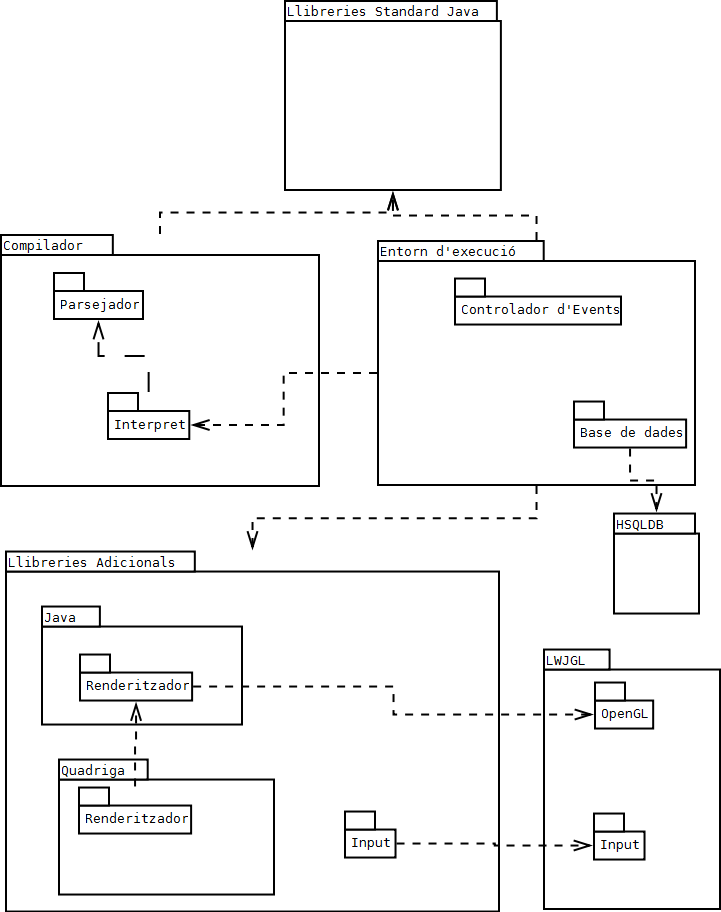
\includegraphics[width=1\linewidth]{./img/Moduls.png}
  \caption{Diagrama de móduls \label{fig:DiagramaDeModuls}}
\end{figure}

Com es veu a la figura \ref{fig:DiagramaDeModuls}, el programa consta d'un {\em compilador}, que a partir d'un seguit de fitxers crea una estructura de dades que posteriorment és interpretada. L'execució necessita d'un {\em entorn}, que s'encarrega essencialment de les operacions pròpies de {\em quadriga} com són la creació, destrucció i cerca de components i entitats, la relació d'un component amb una entitat, l'enviament d'events entre entitats o components, etc\ldots

\section{Model de Dades}

\chapter{Resultats}
\label{chap:Resultats}

  Per tal de validar el sistema funcionava, s'ha provat de fer un joc senzill amb ell, en aquest cas, un clon del Tetris.
  
  El Tetris és un joc creat el 1984, de mecàniques similars a un puzzle i molt conegut arreu del món. La seva simplicitat i la seva fama el fan ideal com a exercici de programació. En podem veure una imatge a la figura \ref{fig:ImatgeTetris}.
  
  \begin{figure}
    \centering
    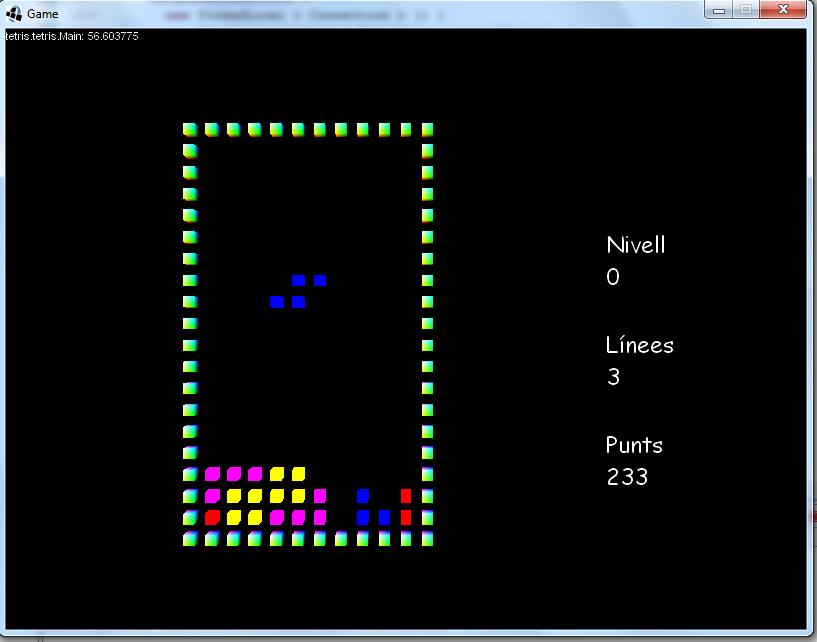
\includegraphics[width=0.5\linewidth]{./img/ImatgeTetris.png}
    \caption{Captura de pantalla del joc final \label{fig:ImatgeTetris}}
  \end{figure}
  
  Les mecàniques del Tetris són molt senzilles: distingim dues entitats bàsiques, el taulell i la peça. La peça cau des de la part superior del taulell, i el jugador pot modificar-ne la trajectòria i girar-la. Un cop la peça no pot descendre més, aquesta queda fixada al taulell i apareix una altra peça a la part superior. Si no pot apareixer aquesta peça, el joc finalitza. Al fixar una peça, pot ser que s'ocupi una línia sencera, en aquest cas s'elimina la línia i es beneficia al jugador amb un seguit de punts.

  En aquest capítol farem un repàs primer dels elements de Quadriga que s'han creat per programar el Tetris, seguidament es farà un cop d'ull a uns elements \"{}estàndard\"{} que s'han creat per tal d'ajudar-ne al desenvolupament. Finalment es farà un anàlisi sobre els objectius de disseny, punt per punt.
  
  \section{Elements propis del Tetris}

    Per tal de veure visualment com està muntat aquest tetris, s'ha fet un diagrama semblant a l'UML de la seva estructura a la figura \ref{fig:TetrisEntitats}. També s'ha confeccionat una llegenda per entendre-ho millor que es pot veure a la figura \ref{fig:GuiaDiagramaQuadriga}.

    \begin{figure}
      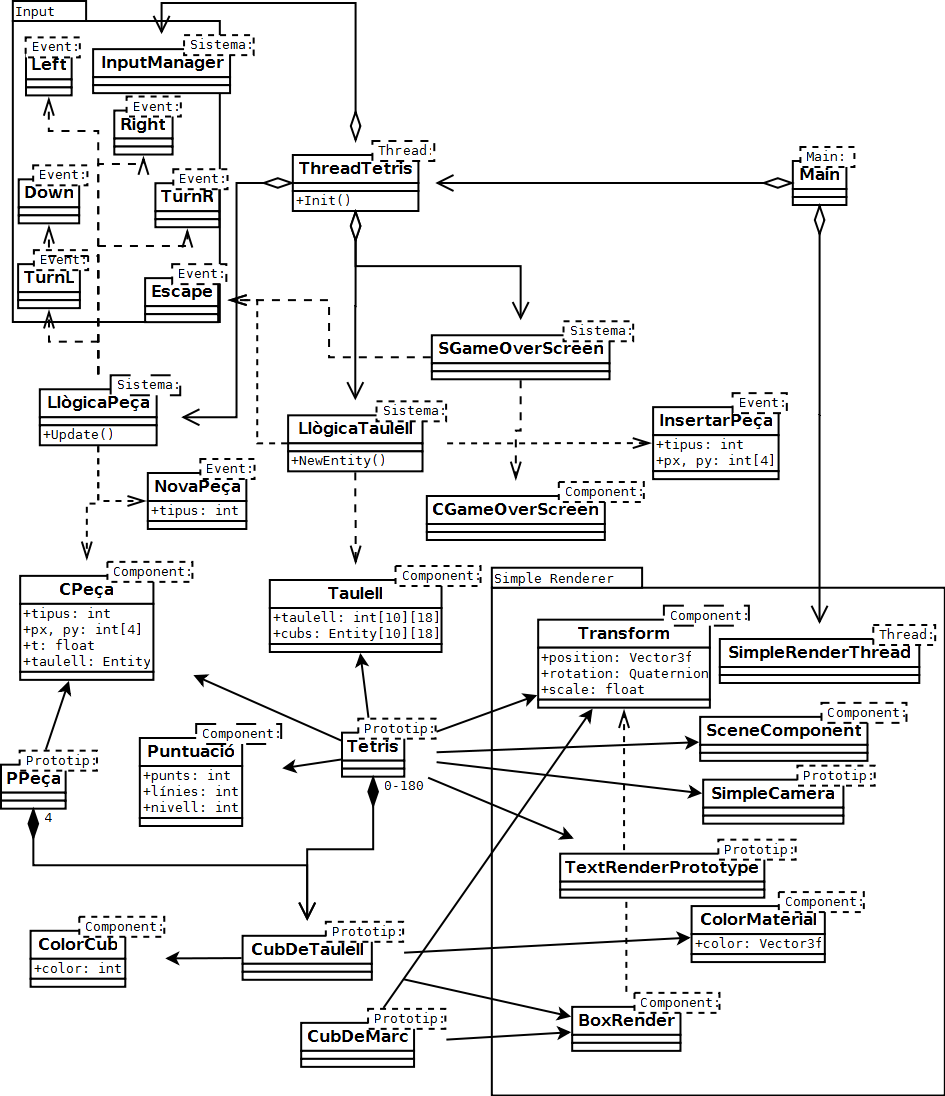
\includegraphics[width=1\linewidth]{./img/TetrisEntitats.png}
      \caption{Esquema dels elements que formen el tetris \label{fig:TetrisEntitats}}
    \end{figure}

    \begin{figure}
      \centering
      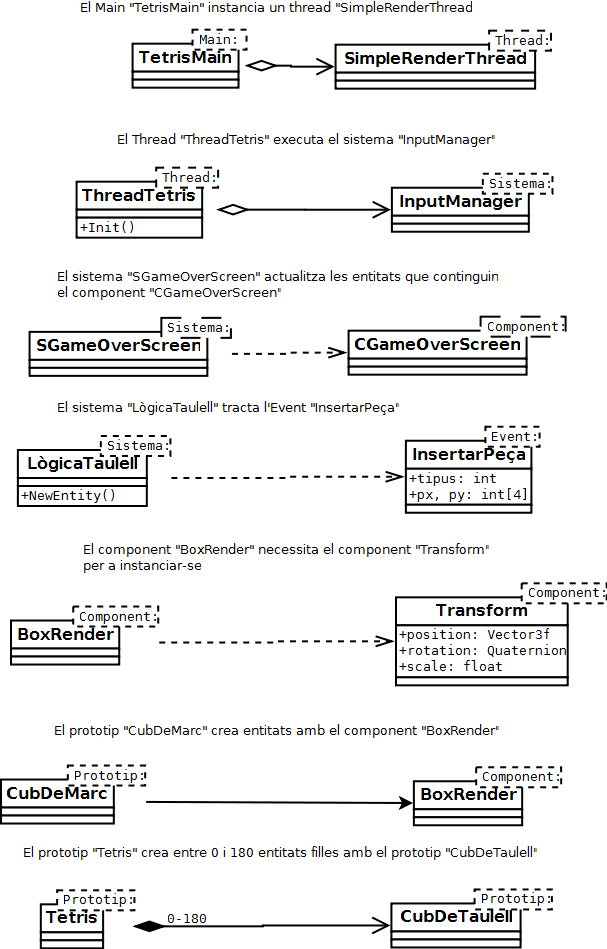
\includegraphics[width=0.7\linewidth]{./img/GuiaDiagramaQuadriga.png}
      \caption{Llegenda \label{fig:GuiaDiagramaQuadriga}}
    \end{figure}

    \subsection{Entitats / Prototips}
      
      \begin{itemize}
        \item {\bf Tetris}
          Representa l'estat actual del taulell de joc, amb els cubs posats, així com també conté informació sobre el nivell actual, els punts i les línies aconseguides pel jugador.
          
        \item {\bf Peça}
          Representa la peça que el jugador ha de col·locar en cada moment. Seria el més semblant a l'Avatar del jugador.
          
        \item {\bf CubDeMarc}
          Representa cada un dels cubs que fan de marc del taulell de joc.
          
        \item {\bf CubDeTaulell}
          Representen els cubs interiors del taulell, tant els col·locats com els que la peça actual aporta. Es diferencien dels anteriors ja que aquests han de tenir un color diferent depenent de la peça.
          
      \end{itemize}

    \subsection{Components}

      \begin{itemize}
        \item {\bf Taulell}
          Guarda informació de quines caselles del taulell estan ocupades per un cub, i en guarda una referència per eliminar-los o moure'ls quan el jugador completa una línia.
          
        \item {\bf Puntuació}
          Guarda informació sobre el nivell, les línies completades i la puntuació feta.
          
        \item {\bf Peça}
          Guarda informació sobre la forma i posició de la peça que actualment cau.
          
        \item {\bf ColorCub}
          Guarda informació sobre el color d'un cub.
          
        \item {\bf GameOverScreen}
          Representa la pantalla final, quan el jugador s'ha rendit o ha perdut.
          
      \end{itemize}

    \subsection{Events}

      \begin{itemize}
        \item {\bf NovaPeça}
          Es crea una nova peça, ja sigui per que s'inicia el joc o s'ha col·locat l'anterior. Aporta informació sobre quin tipus de peça s'ha de crear.
          
        \item {\bf InserirPeça}
          La peça ha arribat a sota i s'ha d'inserir al taulell.
          
        \item {\bf Left, Right, Down, TurnL, TurnR}
          El jugador ha donat instruccions per moure la peça o girar-la.
          
        \item {\bf Escape}
          El jugador ha premut la tecla d'escapament, volent finalitzar el joc o programa.
          
      \end{itemize}

    \subsection{Sistemes}

      \begin{itemize}
        \item {\bf LògicaTaulell}
          Controla la inserció de peces, l'acumulació de punts i si s'han completat línies, augmentant el nivell si s'escau.
          
        \item {\bf LògicaPeça}
          Controla que una peça es mogui segons les ordres del jugador i caigui a una velocitat donada pel nivell actual. També comprova si ha arribat al final i cal inserir-la.
          
        \item {\bf GameOverScreen}
          Un cop el jugador ha acabat la partida, en mostra la puntuació i espera que el jugador doni ordres de tancar el programa.
          
        \item {\bf InputManager}
          Vigila quin input dona el jugador i crea els events corresponents.
          
      \end{itemize}
      
    \subsection{Threads}
    
      \begin{itemize}
        \item {\bf ThreadTetris}
          Inicialitza el joc i executa els 4 sistemes anteriors.
          
      \end{itemize}
    
  \section{Llibreria SimpleRender}

    \subsection{Entitats / Prototips}

      \begin{itemize}
        \item {\bf TextRenderer}
          Renderitza un text donada una {\em Font}, una posició i un {\em String}.
      \end{itemize}


    \subsection{Components}

      \begin{itemize}
        \item {\bf Transform}
          Guarda informació sobre la translació, rotació i escala d'una entitat.
          
        \item {\bf SceneComponent}
          Marca un objecte com a arrel de l'escena.
          
        \item {\bf SimpleCamera}
          Guarda informació sobre la càmera de l'escena.
          
        \item {\bf ColorMaterial}
          L'objecte es renderitza amb un material de color pla.
          
        \item {\bf BoxRender}
          L'objecte es renderitza com una caixa.
          
      \end{itemize}
      
    \subsection{Threads}
    
      \begin{itemize}
        \item {\bf SimpleRenderThread}
          Renderitza tots els objectes de l'escena que contenen algun component \"{}renderitzable\"{} com {\em BoxRender}.
          
      \end{itemize}
      
\section{Objectius de disseny}

  S'analitza, punt per punt, si s'han complert els objectius de disseny del programa.
    
  \begin{figure}
    \centering
    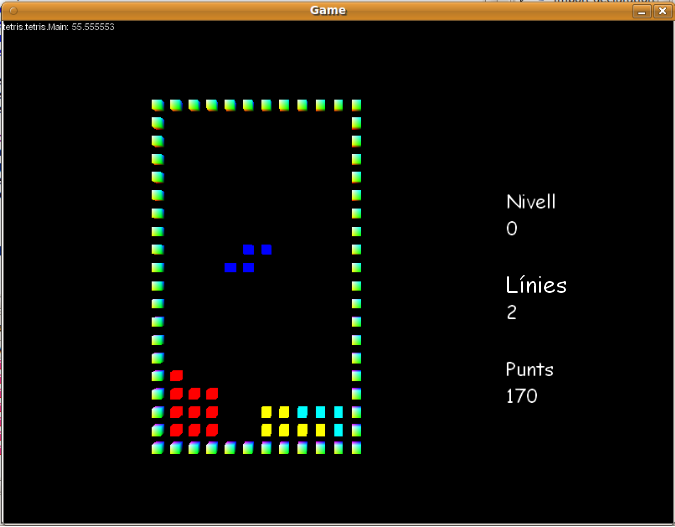
\includegraphics[width=0.5\linewidth]{./img/ImatgeUbuntu.png}
    \caption{Captura de pantalla del joc sobre Ubuntu \label{fig:ImatgeUbuntu}}
  \end{figure}

  \begin{itemize}
    \item {\bf Open Source} \hfill \\
      El codi es pot trobar a \url{https://code.google.com/p/quadriga/} sota llicència {\bf GNU Lesser GPL}.
      
    \item {\bf Independent} \hfill \\
      En l'exemple s'usen unes quantes llibreries Java per implementar aspectes importants del joc. {\em OpenGL} i l'{\em input} del jugador s'obtenen a partir de {\bf LWJGL}. Per fer-les servir des de {\em Quadriga} cal emprar {\em Components} que anomenaríem "estàndard" sota el paquet {\em cat.quadriga.base}. Fer aquests components no és senzill, però es podrien substituir els sistemes si es volgués fer l'esforç sense masses problemes.
      
    \item {\bf Multi-plataforma de forma nativa} \hfill \\
      Com es veu a la figura \ref{fig:ImatgeUbuntu}, el joc corre sobre {\em Ubuntu} sense cap diferència. El codi Java i Quadriga no s'han tocat, però si que cal fer una petita modificació a l'hora de crear l'executable, doncs {\em OpenGL} necessita accedir a llibreries natives que són diferents en cada plataforma.
      
    \item {\bf Permetre un desenvolupament ràpid un cop estiguin fets els components bàsics} \hfill \\
      El codi final són 2 arxius, un de lògica de unes 800 línies i un altre de input de 65. És de fet quasi més llarg fer el disseny que no implementar-lo.
      
      Addicionalment s'ha provat d'afegir funcionalitat. En vint minuts s'ha aconseguit inserir una guia per indicar la peça següent a caure. En total s'han afegit 140 línies (afegir el component, prototip i sistema que controlin la peça següent), de les quals pràcticament totes són una còpia de codi ja fet, i s'han hagut de modificar 3 punts del joc, on s'instanciava una nova peça per tal de fer que agafés el tipus de peça que hi havia guardat. Veure figura \ref{fig:ImatgePecaSeguent}.
      
    \item {\bf Fàcilment paral·lelitzable} \hfill \\
      Actualment el programa conté una opció de fer córrer cada {\em Thread} en paral·lel, però l'opció teòricament òptima de paral·lelitzar l'actualització de cada entitat sobre cada sistema (aconseguint una paral·lelització no sobre el nombre de threads, sinó sobre el nombre d'entitats) no s'ha implementat.
  \end{itemize}
    
  \begin{figure}
    \centering
    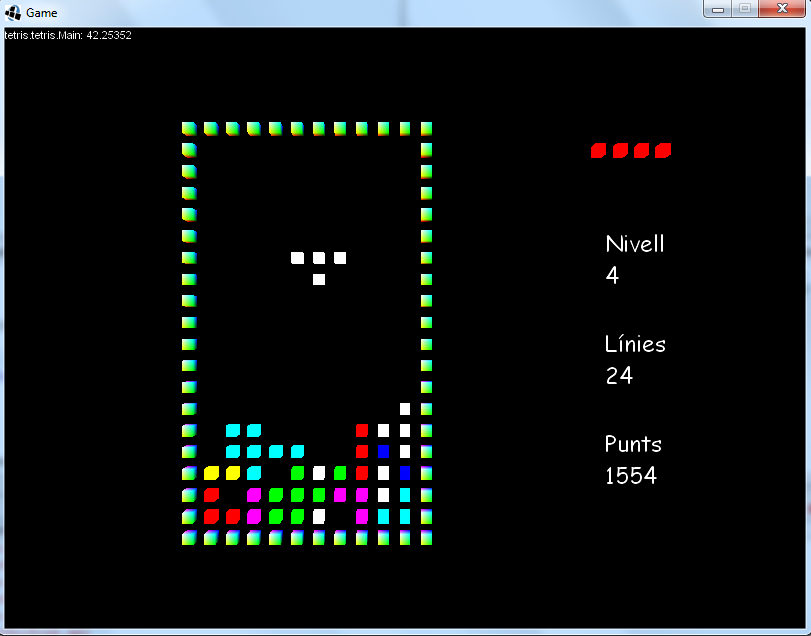
\includegraphics[width=0.5\linewidth]{./img/ImatgePecaSeguent.png}
    \caption{Captura de pantalla del joc amb modificacions \label{fig:ImatgePecaSeguent}}
  \end{figure}

  Per tal de validar els resultats, s'ha considerat que el fet de poder-hi programar-hi un joc consisteix una prova força complerta de que el projecte funciona. S'ha demostrat que el joc es pot ampliar fàcilment, ara es proposaran alguns dissenys de millora:
  
  \begin{itemize}
    \item {\bf Multijugador a pantalla dividida:} Per tal d'implementar aquesta millora, cal duplicar les entitats principals: tenir 2 sistemes i 2 peçes. També cal ampliar els events d'ordres del jugador tal que aportin informació de quin jugador l'ha feta, i que les funcions que responen a aquests events actuin sobre la peça adequada.
    
    \item {\bf Multijugador en xarxa:} Aquesta ampliació és en part més complexa que l'anterior, ja que implica crear un módul de xarxa. Un cop creat aquest módul, les modificacions al programa Quadriga són mínimes, ja que només cal fer que els events que el jugador local crea s'enviin al remot, i fer que els events remots es tradueixin als events locals.
    
    \item {\bf Crear un fons de pantalla més estètic:} Cal crear un component i entitat que ho controlin, així com ampliar la llibreria gràfica. Tot això aniria associat a la llibreria estàndard de Quadriga i les modificacions des del nucli de la lògica serien mínimes.
    
    \item {\em Crear un menú principal, amb pantalla de rècords:} Caldria crear una màquina d'estats que implementés aquest menú. La llibreria estàndard ja incorpora utilitats per renderitzar qualsevol text en {\bf Unicode}. Adicionalment, es podria afegir funcionalitat per guardar l'estat de la base de dades i així mantenir els rècords entre partides.
  \end{itemize}

  

\chapter{Conclusions i Millores}
\label{chap:Conclusions}


\begin{itemize}
  \item S'ha dissenyat un llenguatge de programació que segueix el paradigma dels {\em Sistemes d'Entitats} i s'ha anomenat Quadriga.
  \item S'ha dissenyat i implementat un {\bf compilador} per aquest llenguatge.
  \item S'ha implementat un {\bf entorn d'execució} que proporcioni al programa tots els elements necessaris per al seu correcte funcionament en qualsevol plataforma suportada per Java.
  \item S'ha creat una base de dades especificada dinàmicament (resultat de la compilació) que suporta qualsevol tipus de joc sobre un format estandaritzat.
  \item S'ha creat un subratllador de sintaxi per facilitar la seva programació.
  \item S'ha implementat un joc d'exemple basat en el clàssic {\bf Tetris}.
  \item S'ha desenvolupat una petita llibreria bàsica per a renderitzar textos i algunes formes geomètriques simples: cubs i esferes.
  \item S'ha dissenyat un model de llibreria tal que sigui fàcil de transportar a altres plataformes (fins i tot plataformes mòbils) emprant les últimes tècniques de renderitzat (mitjançant els {\em Shaders} d'OpenGL 2.0).
\end{itemize}

Com a {\bf incidències} importants cal destacar:

\begin{itemize}
  \item La idea d'usar una base de dades {\em SQL} no ha donat resultats massa bons, ja que consumeix molts recursos. Tot i això, es pot fer servir amb poques modificacions per tal de guardar l'estat del joc (funcionalitat de partida guardada) i carregar-lo de forma molt simple.
\end{itemize}

Com a possibles {\bf millores} a aportar al projecte:

\begin{itemize}
  \item Fer que el compilador generi bytecode per executar directament a la màquina virtual de Java, millorant el rendiment dels programes desenvolupats a Quadriga.
  \item Crear una implementació específica del model de dades, sense usar una base de dades SQL. Així el rendiment milloraria considerablement.
  \item Ampliar la llibreria estàndard per incloure la següent funcionalitat:
  \begin{itemize}
    \item Renderitzar formes geomètriques arbitràries (actualment només se suporten cubs, esferes i textos).
    \item Crear una manera de renderitzar models animats per esquelet.
    \item Ampliar els materials per a tenir efectes més complexos.
    \item Afegir funcionalitat de so.
    \item Afegir funcionalitat de joc en xarxa.
  \end{itemize}
  D'aquesta manera el programador o dissenyador tindria més facilitat per desenvolupar-hi jocs.
  \item Crear un plug-in de la {\bf IDE} {\em Eclipse} per a desenvolupar i debugar més fàcilment.
\end{itemize}



\begin{onehalfspace}
\bibliographystyle{ieeetr}
\bibliography{referencies}
\addcontentsline{toc}{chapter}{Bibliografia}
\end{onehalfspace}

\appendix
\newpage
\chapter{El llenguatge Quadriga}
\label{chap:llenguatgeQ}

\section{Estructura dels programes}

Un programa fet amb Quadriga consta de diferents elements (Component, Sistema, Event, Thread, Prototip, Main) distribuïts en diferents fitxers o paquets. El concepte de paquets està directament agafat de {\em Java} i serveix per a crear espais de noms, tal que un programador sigui lliure de crear elements amb el nom que vulgui, que sempre seran compatibles amb altres amb el mateix nom, però diferent paquet.

Cada paquet de Quadriga està representat per un fitxer. Els fitxers de quadriga acaben en {\em \"{}.qdg\"{}}. Si un paquet es diu {\em \"{}tetris.input\"{}} aleshores el fitxer serà anomenat {\em \"{}tetris/input.qdg\"{}}. Aquesta metodologia permet al compilador trobar fàcilment els arxius que necessita. En quadriga no existeix cap ordre per incloure fitxers externs. En comptes d'això, cal declarar els elements que es necessiten, i el compilador els buscarà als directoris d'inclusió. Si per exemple volem fer servir el {\em Component Transform} del paquet {\em cat.quadriga.base} aleshores hem de declarar {\em @component cat.quadriga.base.Transform} abans de fer-lo servir, i el compilador ja s'encarregarà de trobar-lo. Aquesta sentència es pot usar per predeclarar un element del mateix fitxer abans d'on està pròpiament escrit per tal d'utilitzar-lo, de forma similar a com ho fa {\bf C}. Per tal d'importar una classe de {\em Java} cal usar la paraula clau {\bf @java} tal com s'importen la resta d'elements. Com a java, es considera que les classes del paquet {\em java.lang} estan automàticament importades.

El llenguatge utilitza essencialment la mateixa estructura que Java, amb la diferència que a Quadriga no es creen classes, sinó els elements propis: {\em Components, Sistemes, Events, Threads, Prototips i Mains}. També s'han afegit algunes instruccions extres. Totes les paraules clau pròpies de {\em Quadriga} comencen amb el símbol {\bf @}.

\subsection{Entitat}

\begin{verbatim}
Entity<Component1, Component2, ...>
\end{verbatim}

Una entitat, en Quadriga, és simplement un tipus de variable o paràmetre. Com que cada entitat està identificada pels seus components, es permet de nombrar quins components se suposa que té associats de forma similar a com es fan els {\em Generics} en Java.

\section{Declaració de tipus de dades}

\subsection{Components}

\begin{verbatim}
@component Puntuació {
  *CTaulell;
  int punts  = 0;
  int línies = 0;
  int nivell = 0;
}
\end{verbatim}

La declaració d'un Component comença amb la paraula clau {\em \"{}@component\"{}} seguida de l'identificador desitjat del component. Seguidament, dintre de claus (\{ \}), es declaren les variables d'estat de forma similar a Java, amb la possibilitat d'establir un valor inicial si es desitja, tal com es mostra en l'exemple.

També dintre de les claus, i a l'inici es pot especificar quins Components necessita aquest Component (requisits previs), afegint un asterisc {\bf *} i el nom d'aquests components.

Els tipus permesos són els tipus primitius de Java (byte, short, int, long, float, double, boolean, char) i classes que siguin {\em Serialitzables}.

\subsection{Events}

\begin{verbatim}
@event NovaPeça {
  int tipus;
}
\end{verbatim}

Un event es declara de forma idèntica a un component, a excepció de la paraula clau inicial {\em \"{}@component\"{}} que és substituïda per {\em \"{}@event\"{}}; i no hi ha \"{}requisits\"{}.

\subsection{Sistemes}

\begin{verbatim}
@system LògicaPeça {
  @components {
    CPeça
  }
  
  @init {...}
  
  @cleanUp {...}
  
  @update(Entity<CPeça> entitat: ENTITY, float dt : DELTA_TIME) {...}
  
  @newEntity(Entity<CPeça> entitat: ENTITY) {...}
  
  @eraseEntity(Entity<CPeça> entitat: ENTITY) {...}
  
  @event NovaPeça(
                  NovaPeça event: EVENT, 
                  Entity<CPeça> entitat: ENTITY
                  )
  {...}
  
  @event ELeft(Entity<CPeça> entitat: ENTITY) {...}
  
  @event ERight(Entity<CPeça> entitat: ENTITY) {...}
  
  @event EDown(Entity<CPeça> entitat: ENTITY) {...}
  
  @event ETurnL(Entity<CPeça> entitat: ENTITY) {...}
  
  @event ETurnR(Entity<CPeça> entitat: ENTITY) {...}
}
\end{verbatim}

La declaració d'un Sistema comença de forma similar a la d'un component, amb la paraula clau {\em \"{}@system\"{}}, el nom del sistema, i els diferents elements d'aquest. El primer element que cal introduir sempre, i l'únic obligatori, és la llista de components que una Entitat necessita tenir per que aquest sistema l'afecti. Aquesta llista se situa entre les claus de la següent construcció:

\begin{verbatim}
  @components { }
\end{verbatim}

Els elements de la llista poden anar separats de punts i coma ({\bf ;}), però poden estar separats únicament per espais.

A continuació vindran les funcions del sistema. Les dues primeres a destacar són {\bf @init} i {\bf @cleanUp}. Aquestes s'executen a l'inici i a la fi de l'execució, una única vegada. Entre 2 sistemes, l'ordre de en que s'executin aquestes funcions depèn únicament de l'ordre en el qual s'han declarat en un Thread. Si 2 Threads declaren el mateix sistema, aquest s'executarà dues vegades.

La funció més important d'un sistema és normalment la funció {\bf @update}. Aquesta funció s'executa un cop per {\em tick} del joc. En el pas de paràmetres cal comentar la introducció del concepte de {\bf semàntiques}. Aquestes semàntiques s'indiquen després de cada paràmetre usant el símbol dos punts {\bf :}. El tipus de paràmetre cal que sigui compatible amb la semàntica. En el cas de la funció {\bf @update} se'n proporcionen 2:

\begin{itemize}
  \item {\bf ENTITY}: Correspon a la entitat actualitzada.
  \item {\bf DELTA\_TIME}: És el temps, en segons, des de la última vegada que es va cridar la funció per la mateixa entitat.
\end{itemize}

Les següents funcions són {\bf @newEntity} i {\bf @eraseEntity}, que es criden quan una entitat té per primera vegada els components necessaris o deixa de tenir-los, respectivament. Aquestes funcions només proporcionen la semàntica {\bf ENTITY}.

Finalment hi ha les funcions que tracten events. Aquestes funcions comencen amb la paraula clau {\bf @event}, seguida de l'identificador de l'event que es vol tractar. Quan una entitat que pertany al sistema rebi l'event, automàticament es cridarà aquesta funció. A part de la semàntica {\bf ENTITY}, es proporciona la semàntica {\bf EVENT}, que ha de tenir el mateix tipus que l'event tractat i proporcionarà totes les dades que vinguin amb aquest event.

\subsection{Prototips}

\begin{verbatim}
@prototype PPeça(Entity<Puntuació> taulell)
{
  Transform()
  CPeça(taulell: taulell)
  @child {
    "cub1" : CubDeTaulell(posX:0, posY:0, color: 1)
    "cub2" : CubDeTaulell(posX:0, posY:0, color: 1)
    "cub3" : CubDeTaulell(posX:0, posY:0, color: 1)
    "cub4" : CubDeTaulell(posX:0, posY:0, color: 1)
  }
}
\end{verbatim}

L'estructura d'un prototip és una mica més complexa. Primer cal especificar-ne el nom, seguit dels paràmetres que té el prototip. Després se li afegeixen un seguit de plantilles per a dues coses: Components que tindrà l'entitat, i altres entitats filles que crearà. Els elements sempre es creen i afegeixen en l'ordre establert.

Per a afegir un component, simplement cal escriure el nom i, entre parèntesi, donar valor als camps. Per fer-ho, només cal escriure el nom del camp, dos punts {\bf :} i el valor a assignar-hi. Aquells camps que tinguin valor per defecte no cal que siguin assignats.

Per a especificar Entitats filles, cal especificar-les dintre d'una estructura {\em\"{}@child\{ \}\"{}}. Aquí la fòrmula a utilitzar és indicar primer el nom (de forma opcional), a continuació el prototip utilitzat i finalment els paràmetres, de forma similar als Components. Si es vol sobreescriure un valor d'un Component d'algun d'aquests fills, s'haurà d'especificar el nom del component, punt {\bf .} i finalment el camp del component.

Finalment també es pot executar codi si aquest va dintre d'una estructura {\em\"{}@init\{ \}\"{}}, que pot ser repetida diverses vegades al prototip.

\subsection{Threads}

\begin{verbatim}
@thread LlogicaTetris {
  @system SGameOverScreen;
  @system InputManager;
  @system LlògicaTaulell;
  @system LlògicaPeça;
  
  @init {...}
  
  @cleanUp {...}
}
\end{verbatim}

Un Thread indica quins Sistemes s'executaran, i en quin ordre, i una funció d'Init i CleanUp (opcionals) que s'executaran a l'inici i final de l'execució del programa.

\subsection{Main}

\begin{verbatim}
@main Main {
  @thread SimpleRenderThread
  @thread LlogicaTetris
  
  @init {...}
  
  @cleanUp {...}
}
\end{verbatim}

L'objecte Main indica quins Threads s'executen i l'ordre d'aquests (si l'execució no és paral·lela), a més d'un Init i un CleanUp.

\section{Instruccions pròpies}

\subsection{Nova Entitat}

\begin{verbatim}
@newEntity(nom, pare)
\end{verbatim}

Aquesta instrucció retorna una Entitat nova. Se li pot especificar un nom i una Entitat pare, o deixar els paràmetres a null.

\subsection{Eliminar Entitat}

\begin{verbatim}
@eraseEntity entitat;
\end{verbatim}

Elimina una Entitat.

\subsection{Cercar Entitat}

\begin{verbatim}
@find[nom]
\end{verbatim}

Cerca una Entitat amb el nom especificat i sense pare.

\subsection{Aplicar prototip}

\begin{verbatim}
@prototype entitat : nomPrototip( param1: valor1, param2: valor2, 
                                  Component1.camp1: valor3, Component1.camp2: valor4,
                                  ...)
\end{verbatim}

Fa que a una Entitat se li apliqui un Prototip.

\subsection{Agregar Component}

\begin{verbatim}
@add nomComponent(param1: valor1, param2: valor2) : entitat;
\end{verbatim}

Fa que a una Entitat se li agregui un Component.

\subsection{Cridar Event}

\begin{verbatim}
@event[temps] nomEvent(param1: valor1, param2: valor2) : entitat ;
\end{verbatim}

Crida un event. El temps ha de ser positiu, o es pot ometre (per fer una crida instantània), així com la Entitat sobre la que cridar també es pot ometre (fent un Broadcast).

\subsection{Accedir a un Component}

\begin{verbatim}
entitat[Component]
\end{verbatim}

Accedeix a un Component de la Entitat.

\subsection{Accedir a una Entitat filla}

\begin{verbatim}
entitat["nomFilla"]
\end{verbatim}

Accedeix a una Entitat filla amb el nom especificat.

\subsection{Nombre Aleatori}

\begin{verbatim}
@rnd
\end{verbatim}

Retorna un objecte del tipus {\em java.util.Random}.

\section{Execució}

Per executar un programa de quadriga cal executar la classe {\em cat.quadriga.parsers.Quadriga} amb un únic paràmetre: el nom de l'objecte Main que es vol executar. Cal que Java pugui trobar totes les llibreries Java necessàries (vecmath, hsqldb, lwjgl, slick-util, lwjgl-util) com les llibreries natives de LWJGL.
\chapter{El projecte Quadriga}

El projecte, amb el codi font i alguns exemples, es pot trobar a la pàgina \url{http://quadriga.googlecode.com}. Addicionalment també es pot trobar aquesta mateixa memòria. En el moment d'escriure aquesta memòria, el projecte es pot aconseguir d'un servidor de {\bf Subversion}, actualment a la revisió número 100. El codi està pensat per a ser compilat amb la {\em IDE Eclipse} de la següent manera:

\begin{enumerate}
  \item Cal instal·lar Eclipse amb els plugins {\em subclipse} \url{http://subclipse.tigris.org/} i {\em JavaCC Eclipse Plug-in} \url{http://eclipse-javacc.sourceforge.net/}.
  
  \item Cal descarregar el projecte {\bf SVN} des d'Eclipse amb repositori a \url{http://quadriga.googlecode.com/svn/trunk/Quadriga Parser/}. \\
        Alternativament es pot descarregar tot el projecte amb {\bf SVN} ja sigui amb la consola o usant un programa com {\bf Tortoise SVN} \url{http://tortoisesvn.tigris.org/}.
        
  \item Descarregar les llibreries {\bf LWJGL} \url{http://lwjgl.org/download.php} i {\bf HSQLDB} \url{http://sourceforge.net/projects/hsqldb/files/}. 
        Incloure ambdues llibreries al projecte d'Eclipse (figura \ref{fig:incloure}).
        
  \item Finalment cal indicar-li a l'Eclipse on troba les llibreries dinàmiques de {\bf LWJGL} (figura \ref{fig:incloure3}).
\end{enumerate}

\begin{figure}
  \centering
  \subfloat[Obrir les propietats del projecte]{\label{fig:incloure1}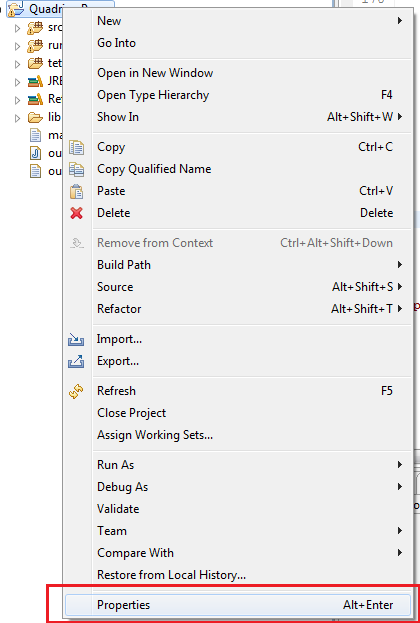
\includegraphics[width=0.48\textwidth]{./img/incloure1.png}}                
  \subfloat[Afegir els les llibreries (jar) necessàries]{\label{fig:incloure2}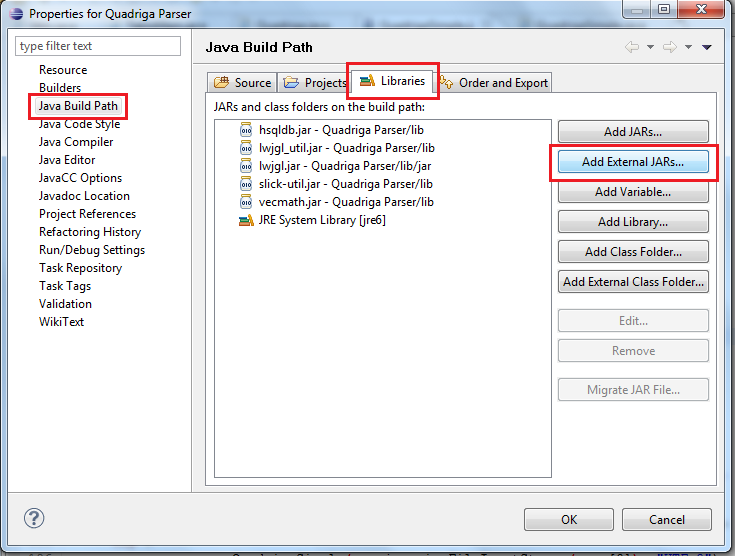
\includegraphics[width=0.48\textwidth]{./img/incloure2.png}}
  \caption{Com incloure les llibreries necessàries}
  \label{fig:incloure}
\end{figure}

\begin{figure}
  \centering
  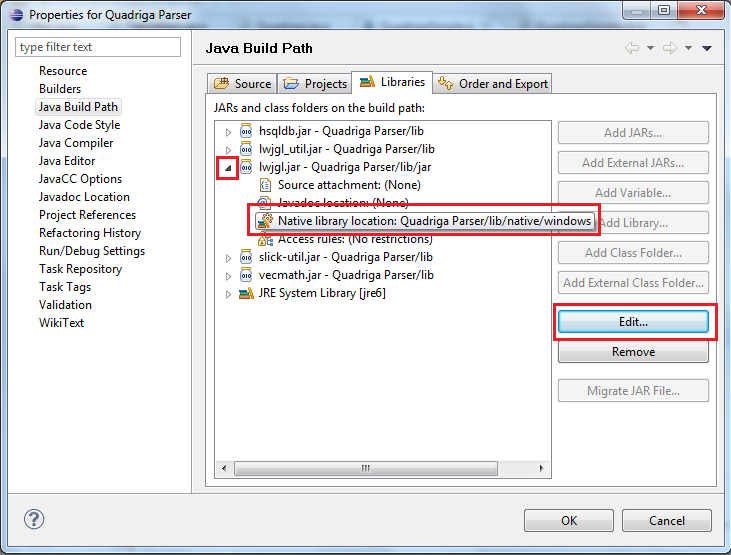
\includegraphics[width=0.58\linewidth]{./img/incloure3.png}
  \caption{Indicar-li el path a les llibreries dinàmiques \label{fig:incloure3}}
\end{figure}

\newpage
\pagestyle{empty}

\begin{onehalfspace}

{\bf RESUM:} Aquest projecte tracta del desenvolupament d'una plataforma on crear la lògica de videojocs. S'ha decidit crear un llenguatge especial per a descriure aquesta lògica i per fer-ho s'ha seguit l'arquitectura del \"{}Sistemes d'Entitats\"{}, ja que és una arquitectura que s'ha anat desenvolupant al llarg dels anys dins del mateix sector dels videojocs. Per a fer-ho s'ha creat un analitzador sintàctic i un generador de codi, així com un intèrpret i un entorn d'execució. Addicionalment s'hi ha afegit una llibreria que proveeixi els altres mòduls necessaris per desenvolupar un videojoc i s'ha implementat el Tetris a mode de prova i exemple.
\\

{\bf RESUMEN:} Este proyecto trata del desarrollo de una plataforma donde crear la lógica de videojuegos. Se ha decidido crear un lenguage especial para describir esta lógica y para ello se ha usado la arquitectura de \"{}Sistema de Entidades\"{}, ya que es una arquitectura que se ha desarrollado a lo largo del tiempo dentro de la misma industria de los videojugos. Para ello se ha creado un analizador sintáctico y un generador de código, además de un intérprete y un entorno de ejecución. Adicionalmente se ha añadido una librería que provea los otros módulos necesarios para el desarrollo de un videojugo y se ha implementado el Tetris a modo de prueba y ejemplo.
\\

{\bf ABSTRACT:} This project is about the development of a platform where one can create the logic of a video game. To do so, a language has been created to describe this logic using the architecture known as \"{}Entity System\"{}, because this architecture was developed in the video game industry itself. In order to accomplish that, a parser and a code generator have been created, also a code interpreter and an execution environment have been added. In order to have all the needed functionality to create a video game, a standard library has been developed and a Tetris Clone was created as a test and example.

\end{onehalfspace}


\end{document}
